%%%%%%%%%%%%%%%%%%%%%%%%%%%%%%%%%%%%%%%%%
% "ModernCV" CV and Cover Letter
% LaTeX Template
% Version 1.11 (19/6/14)
%
% This template has been downloaded from:
% http://www.LaTeXTemplates.com
%
% Original author:
% Xavier Danaux (xdanaux@gmail.com)
%
% License:
% CC BY-NC-SA 3.0 (http://creativecommons.org/licenses/by-nc-sa/3.0/)
%
% Important note:
% This template requires the moderncv.cls and .sty files to be in the same 
% directory as this .tex file. These files provide the resume style and themes 
% used for structuring the document.
%
%%%%%%%%%%%%%%%%%%%%%%%%%%%%%%%%%%%%%%%%%

%----------------------------------------------------------------------------------------
%	PACKAGES AND OTHER DOCUMENT CONFIGURATIONS
%----------------------------------------------------------------------------------------

\documentclass[11pt,a4paper,sans]{moderncv} % Font sizes: 10, 11, or 12; paper sizes: a4paper, letterpaper, a5paper, legalpaper, executivepaper or landscape; font families: sans or roman

\moderncvstyle{banking} % CV theme - options include: 'casual' (default), 'classic', 'oldstyle' and 'banking'
\moderncvcolor{blue} % CV color - options include: 'blue' (default), 'orange', 'green', 'red', 'purple', 'grey' and 'black'

\usepackage[utf8]{inputenc}
\usepackage[T1]{fontenc}
\usepackage{lipsum} % Used for inserting dummy 'Lorem ipsum' text into the template
\usepackage{parcolumns}
\usepackage{comment}

\usepackage[top=0.8cm, bottom=1cm, left=1.5cm, right=1.5cm]{geometry} % Reduce document margins
%\setlength{\hintscolumnwidth}{3cm} % Uncomment to change the width of the dates column
%\setlength{\makecvtitlenamewidth}{10cm} % For the 'classic' style, uncomment to adjust the width of the space allocated to your name

\definecolor{color1}{rgb}{0.22,0.45,0.70}% light blue
%----------------------------------------------------------------------------------------
%	NAME AND CONTACT INFORMATION SECTION
%----------------------------------------------------------------------------------------

\firstname{Andrea} % Your first name
\familyname{BRUGNOLI} % Your last name

%% All information in this block is optional, comment out any lines you don't need
%\address{Via Ca' del Frate 7 E}{Negrar (VR), Italy 37024}
%\mobile{(+39) 340 8323361}
%% \phone{(000) 111 1112}
%% \fax{(000) 111 1113}
%\email{brugnoss.ab@gmail.com}
%% \homepage{staff.org.edu/~jsmith}{staff.org.edu/$\sim$jsmith} % The first argument is the url for the clickable link, the second argument is the url displayed in the template - this allows special characters to be displayed such as the tilde in this example
%\extrainfo{Skype contact: brugnoss}
%\photo[70pt][0.4pt]{pictures/Foto_cv} % The first bracket is the picture height, the second is the thickness of the frame around the picture (0pt for no frame)

\AtBeginDocument{\hypersetup{baseurl={}}}

%----------------------------------------------------------------------------------------

\begin{document}

%\makecvtitle % Print the CV title

\begin{minipage}{.8\linewidth}
{\huge{\textsc{Andrea BRUGNOLI} }}

\vspace{2mm}
{1 Avenue de Rangueil, 31400 Toulouse (FR)}

{(+33) 7 50 39 47 27}

{Andrea.BRUGNOLI@supaero.isae.fr or andrea.brugnoli92@gmail.com}

\vspace{3mm}
% \homepage{staff.org.edu/~jsmith}{staff.org.edu/$\sim$jsmith} % The first argument is the url for the clickable link, the second argument is the url displayed in the template - this allows special characters to be displayed such as the tilde in this example
%\end{minipage}
%\begin{minipage}{.4\linewidth}

\fcolorbox{cyan}{white}{%
    \parbox{\textwidth}{\textbf{Ingénieur aérospatial} \newline
Politecnico di Milano (Milano)/ ISAE-Supaero (Toulouse)   \newline
  Doté d'un esprit international, d'initiative et capable de s'adapter. Trois langues maîtrisées. 
  }}
\end{minipage}
\begin{minipage}{.2\linewidth}
\begin{center}
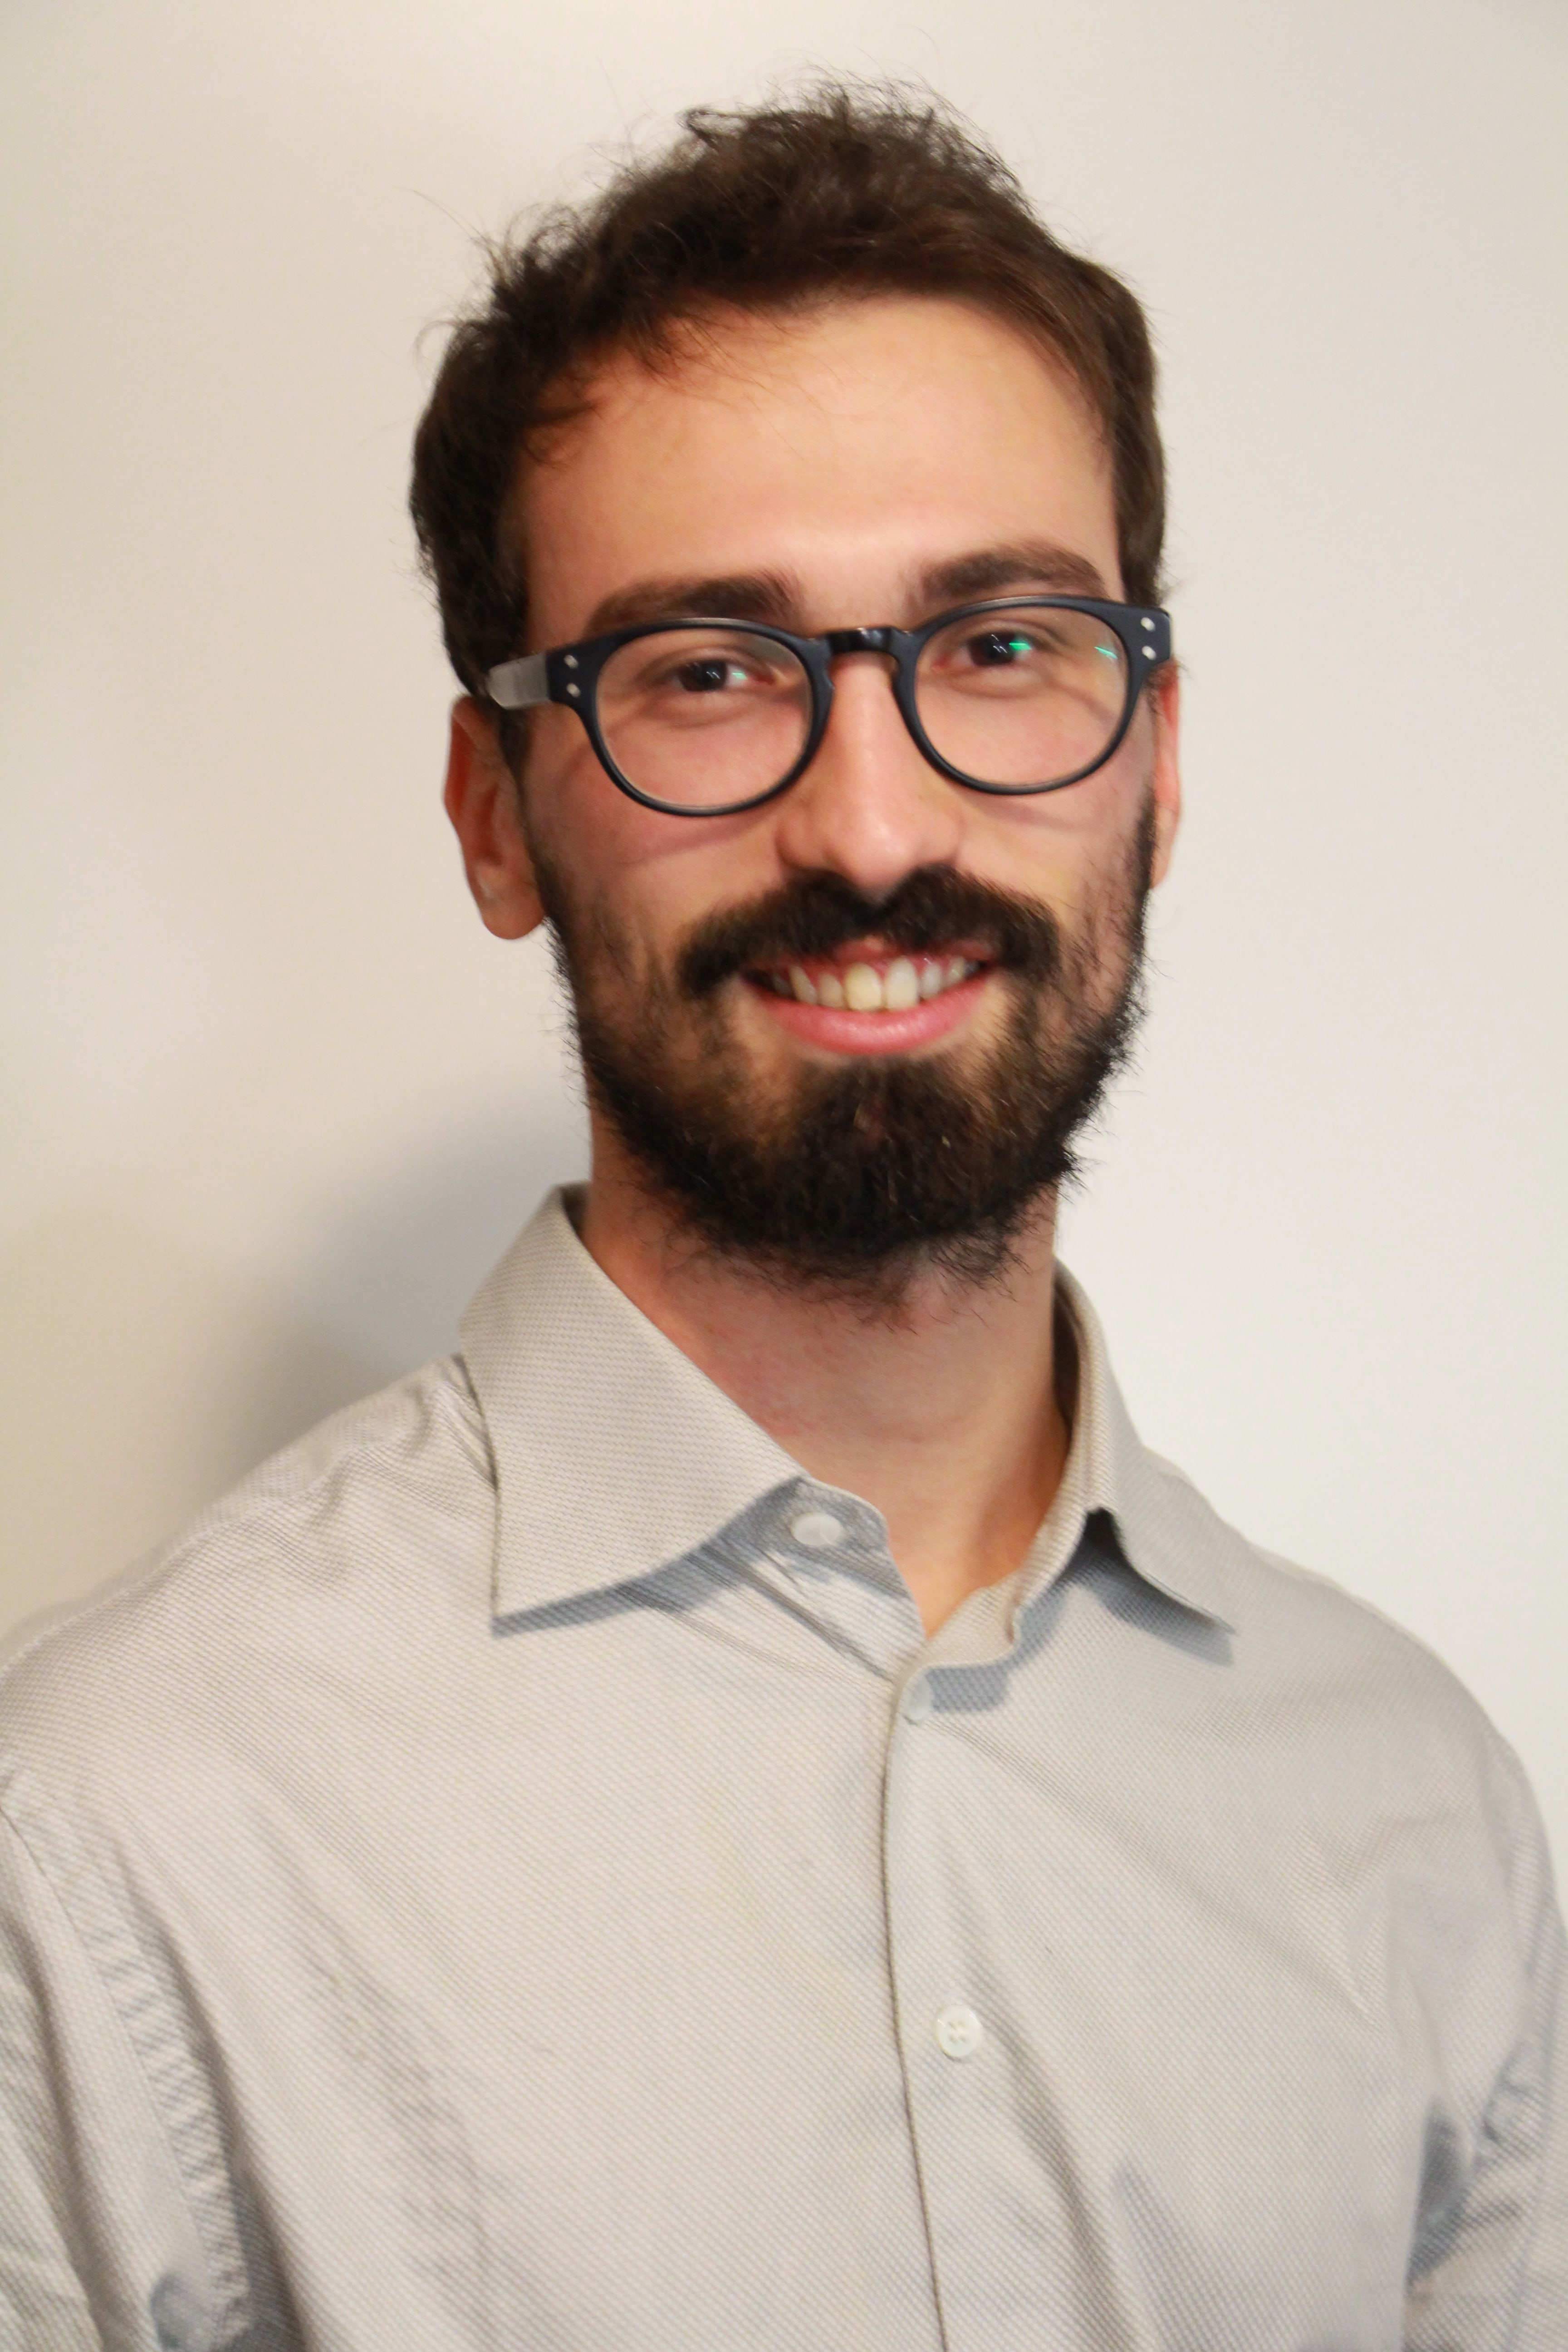
\includegraphics[width=0.8\linewidth]{Foto_Cv-min.jpg}
\end{center}
\end{minipage}

\vspace{2mm}
%\textbf{\'A la recherche d'une position mois à partir de octobre 2017}

%----------------------------------------------------------------------------------------
%	EDUCATION SECTION
%----------------------------------------------------------------------------------------

\vspace{1mm}



\section{Formation académique}

\cventry{2017, 3 ans}{Thèse}{ISAE-Supaero}{Toulouse}{}{Modélisation et Contrôle par le formalisme pHs des structures flexibles 2D avec des conditions aux limites variantes}
% usage: \cventry[spacing]{years}{degree/job title}{institution/employer}{localization}{optionnal: grade/...}{optional: comment/job description}

\cventry{2016--2017}{Master recherche en automatique et traitement d'images}{Université Paris Saclay/\,Supélec}{Paris/Toulouse}{}{Modules: identification des modèles, dynamique avancée des structures flexibles}

\cventry{2015--2017}{Double Diplôme en génie aéronautique et aérospatial}{ISAE-Supaero}{Toulouse}{}{Spécialisation mathématiques appliques et automatique avancée: optimisation multidisciplinaire, calcul hautes performances, systèmes non linéaires et calcul de trajectoires optimales}


\cventry{2014--2017}{Master en génie spatial}{Politecnico di Milano}{Milan}{\textit{110/110 avec mention}}{Modules : Mécanique orbitale, dynamique et contrôle des structures, propulsion thermochimique}


\cventry{2011--2014}{Licence en génie mécanique}{Politecnico di Milano}{Milan}{\textit{110/110 avec mention} }{Modules : méthode des éléments finis, vibrations mécaniques, calcul numérique }

%\cventry{2006--2011}{Baccalauréat Littéraire}{Liceo Classico Scipione Maffei}{Verona}{\textit{100/100}}{}

%\vspace{1mm}

%----------------------------------------------------------------------------------------
%	WORK EXPERIENCE SECTION
%----------------------------------------------------------------------------------------

\section{Expériences}

\cventry{2017, 6 months}{Stage fin études}{CNES-Centre  des études spatiales}{Toulouse}{}{Analyse des débris spatiaux soumis à la pression de radiation solaire pour identifier configurations périodiques en attitude ou stable en pointage}


\cventry{2016, 5 mois}{Téléopérations intelligents pour systèmes des micro-drones}{ISAE-Supaero en partenariat avec LAAS}{Toulouse}{}{Codage des lois de commande optimal en C/C++ pour micro-drones engagés en tâches complexes. Équipe de 6 personnes.}

\cventry{2016, 4 mois}{Dynamique non linéaire des systèmes multi-corps}{ISAE-Supaero}{Toulouse}{}{Modélisation d'une chaîne ouverte des corps en suivant la logique de Simscape Multibody. Validation en Matlab.}

%\cventry{2015, 2 mois}{Transfert interplanétaire}{Politecnico di Milano}{Milan}{}{Étude des trajectoires optimales  avec assistance gravitationnelle pour la minimisation du propergol utilisé. Analyse des perturbations.}

\cventry{2014, 4 mois}{Dynamique d'un manipulateur pour machines de forgeage}{Politecnico di Milano en partenariat avec Danieli S.p.A }{Milan}{}{Étude des dessins techniques, modélisation cinématique et analyse dynamique. Présentation chez Danieli (Septembre 2014).}

%\cventry{}{Design d'une éolienne é axe horizontal  }{Politecnico di Milano}{Milano}{}{Dimensionnement général, optimisation performance au point nominal, analyse de performance hors design. équipe de quatre personnes. Publié sur Academia  \textcolor{blue}{\texttt{\href{https://www.academia.edu/9561531/Horizontal_Axis_Wind_Turbine_Design}{Horizontal Axis Wind Turbine Design}}} }

\cventry{2014, 4 mois}{Analyse é éléments fins d'une pièce mécanique}{Politecnico di Milano}{Milan}{}{Implantation sur Abaqus et codage en Matlab d'un modèle équivalent, validation et comparaison des résultats.}


%----------------------------------------------------------------------------------------
%	COMPUTER SKILLS SECTION
%----------------------------------------------------------------------------------------

%----------------------------------------------------------------------------------------
%	COMMUNICATION SKILLS SECTION
%----------------------------------------------------------------------------------------

% \section{Communication Skills}

% \cvitem{2010}{Oral Presentation at the California Business Conference}
% \cvitem{2009}{Poster at the Annual Business Conference in Oregon}

%----------------------------------------------------------------------------------------
%	LANGUAGES SECTION
%----------------------------------------------------------------------------------------
\begin{minipage}[t]{0.4\linewidth}
\section{Langues}
\cvitem{Anglais}{courant (C1) (Toeic 965/990 2014)}
\cvitem{Français}{courant (C1)}
\cvitem{Espagnol}{intermédiaire (B1)}
\cvitem{Italien}{langue maternelle}
\end{minipage}
\begin{minipage}[t]{0.55\linewidth}
\section{Compétences informatiques}
\cvitem{Programmes}{Matlab, Simulink, Abaqus, Inventor, Solid Works, Labview }
\cvitem{Langages}{ Java, C, C++, \LaTeX}
\end{minipage}


%\cvitem{Italien}{Langue maternelle}{} \cvitem{Anglais}{Niveau courant : Toeic 965/990 (2014)}{}
%\cvitem{Franéais}{Niveau courant} {} \cvitem{Espagnol}{Niveau débutant} {}

%----------------------------------------------------------------------------------------
%	INTERESTS SECTION
%----------------------------------------------------------------------------------------

\section{Centres d'intérêt}

\cvitem{}{Professeur particulier de mathématiques et physique niveau Bac+1 Bac+2}
%\cvitem{}{ Tennis, voyages, cinéma, littérature}

\end{document}